\clearpage
\section{Introduction}

Various types of road damage may occur due external factors such as weather and traffic load. For example, freezing and thawing of asphalt causes cracks. Repeated traffic loads causes asphalt to fatigue and rutting occurs, which is when the pavement surface is deformed along the wheel paths. Poor road surface condition causes discomfort for drivers and more importantly, imposes safety risks. In addition, roads play a vital part in the economic infrastructure of a country, by providing access to education, health and employment services. Adequate routine maintenance prevent major repairs and extend the life of the road, which also safes costs for the maintainer. Conventionally, visual and manual methods are adopted to assess the state of roads. However, they are generally subjective, tedious, labor-intensive, and time consuming. 

To address these difficulties, automated detection methods have been developed by various private companies and researches. Most commonly researched are image based methods to automatically identify damages \cite{Jahanshahi2012,Zhang2016}. Images can be complemented by depth information through infrared sensors or LIDAR \cite{Zhang2017}, which also mitigates image specific drawbacks such as lightning and shadows. More recently researchers use low-cost sensors such as smartphones to automatically detect road damages \cite{Chatterjee2018,Maeda2018,Maeda2020}. Accelerometers, which measure vibrations, have also been used to assess the pavement quality \cite{Hanson2014,Buttlar2014,Gupta2020}. 

In the Netherlands, public infrastructure maintainers (i.e., the state, provinces, municipalities, and water authorities) have the legal responsibility for maintaining their assets. Maintaining is defined by law as ``ensuring that all roads within the area are in good condition'' \cite{Wegenwet}. Road maintainers are obliged to maintain facilities regularly and in a sustainable way \cite{BurgerlijkWetbook6:174}. In order to give some guidance on how to assess the state of roads, standards are made by the national knowledge platform ``CROW''. Among its activities, CROW prescribes road maintainers how to perform road inspections \cite{CROW_147} to help maintainers in quality-driven asset management. 

Road maintenance is a big expenditure of the state's budget, it is annually around 2.5 - 3.5 billion EUR \cite{Rijksbegroting:Infrastructuur}. Depending on the type of the road, a different type of government is responsible for the maintenance. For instance, highways (indicated with A) are maintained by the state, provincial roads (indicated with N) by the provinces, and local roads (indicated with street names) by municipalities. Public bodies are legally obliged to report ``maintenance capital goods'' in their annual budgets \cite{Wet_Besluit_Begroting}. Within the report they have to state the policy framework for maintenance and the financial implications. Road maintenance is planned through a multi-year plan, which requires clear insights in current road conditions. 

\begin{figure}[ht]
    \begin{center}
    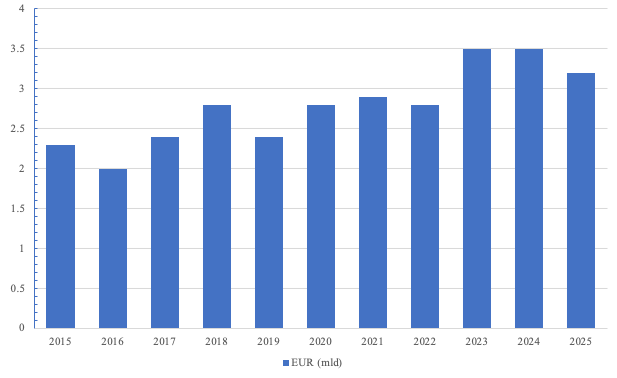
\includegraphics[height=6cm]{images/1_introduction/budget.png}
    \end{center}
    \caption{Budget for maintenance of public roads \cite{Rijksbegroting:Infrastructuur}. Budget is in billion EUR.}
    \label{fig:prm}
\end{figure}

Road maintenance is performed according to an annual cyclical process. The road owner or maintainer (i.e., state, province or municipality) initiates a tender for inspection. After which, an inspection company inspects the road with specialized vehicles. This vehicle contains multiple cameras to record the road surface, infrared sensor to measure the evenness, and other types of sensors. The recorded video data is manually inspected by engineers according the prescribed CROW method \cite{CROW_147}. The inspection company delivers a report with recommendations to the road owner indicating which roads needs maintenance. On this recommendation, the road owner initiates another tender to perform the actual maintenance. Interestingly to note is that companies that can perform inspections, often also can perform the construction.

The condition of the road is measured through various quantifiable data sources. These sources are manually inspected according to CROW method to assess the state of the road. Below is a list given of data sources which are often used within the Netherlands for road inspection:
\begin{itemize}
\item Visual inspection: video data is manually annotated to mark damages.
\item ARAN measurements: laser sensor which measures distance between the road and vehicle across the pavement, and can be used to measure the surface unevenness or rutting.
\item Ground penetrating radar: geophysical method which uses radar pulses to get an image of the subsurface by measuring the reflected signals to assess the quality of the asphalt and deeper layers, detect sinkholes and objects below the surface.
\item Falling weight deflector: similar to ground penetrating radar, but using radar pulses, a weight is dropped and reflections are measured. This method is more commonly used in civil engineering. 
\item Skid resistance: describes the force when a locked tire (i.e., a wheel that is prevented from rotating) slides along the surface. Measurements are performed by measuring the friction on the locked wheel to detect if the road is too slippery leading to aquaplaning.
\item Static data:  besides actual measurements, there is also static data on roads such as:
\begin{itemize}
\item Materials passport describing the different layers of the road. Contains information when and how a layer was constructed and which material was used.
\item Historical maintenance reports.
\item Future date of maintenance (i.e., multi-year plan). 
\item Road intensity (i.e., how many vehicles travel the road).
\end{itemize}
\end{itemize}

Keeping track of these various sources of data is cumbersome. Although many road owners manage this data manually, there are some tools to support their workflow. These software tools are known as ``asset management software'' or ``management systems''. One of the available tools on market is Predictive Road Maintenance (PRM), a platform for data driven asset management (see figure \ref{fig:prm}) developed by AssetWorx\footnote{Pronounced as Asset Works}, where the use cases of this thesis is derived. PRM was initially developed during an incubator program known as ``Startup in Residence'' funded by the Overijssel province \cite{Residense2020}. The goal of AssetWorx is to create an uniform data platform for asset management. The idea is to be a industry disrupter by providing data driven insights concerning road quality, maintenance and planning as an independent organization. 

\begin{figure}[ht]
    \begin{center}
    \includegraphics[width=0.8\textwidth]{images/1_introduction/prm-overview.png}
    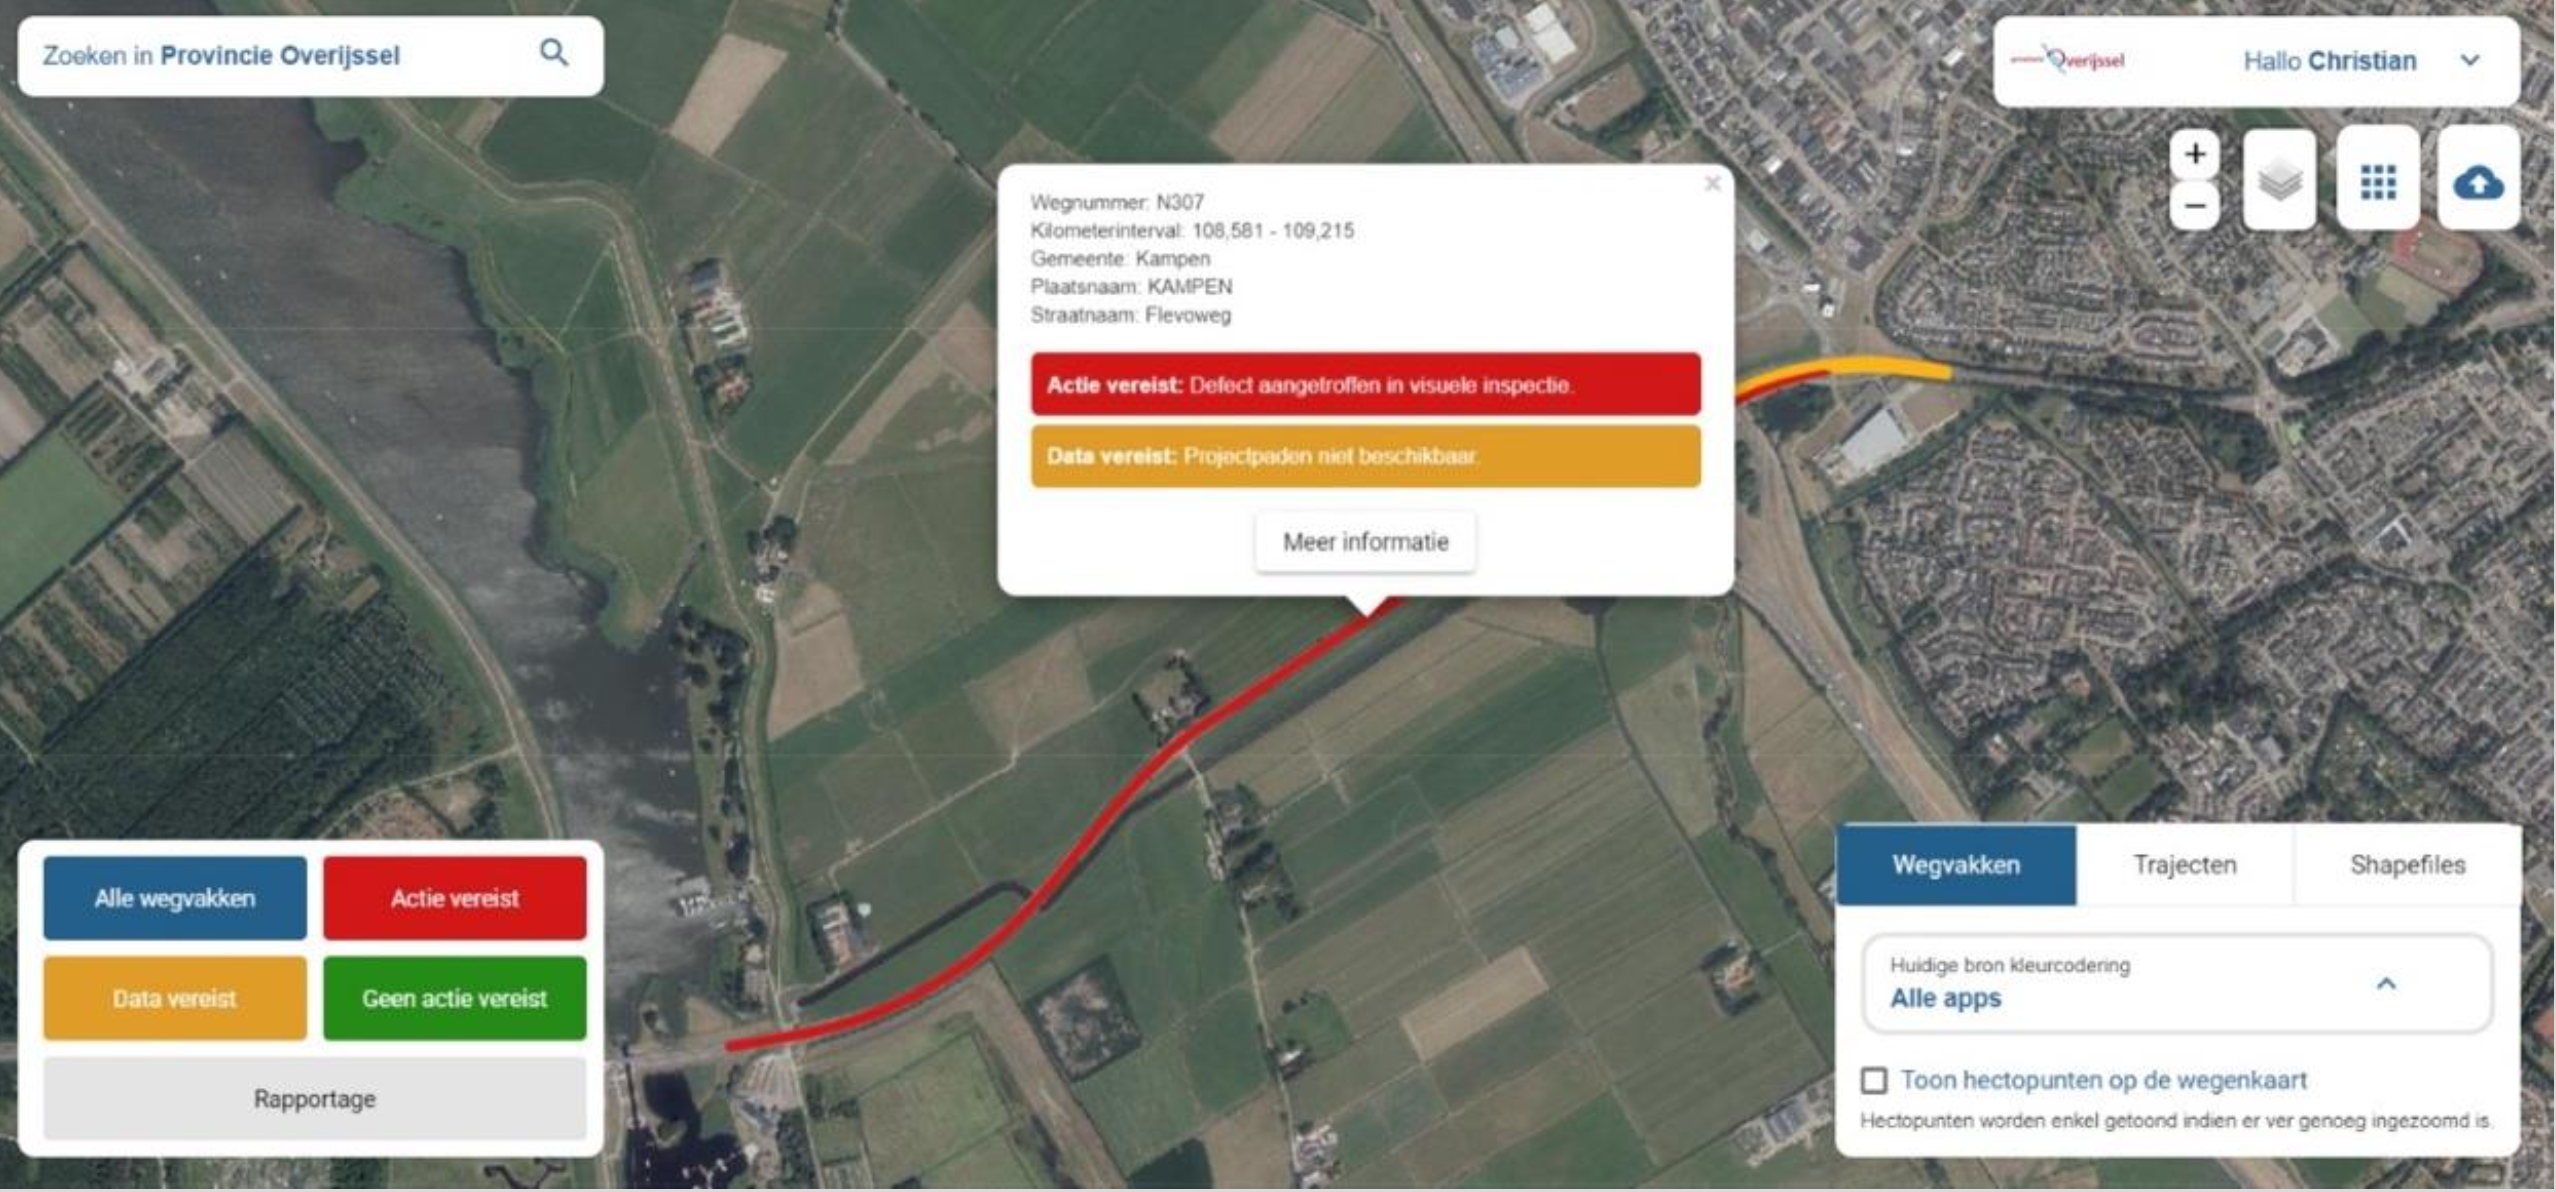
\includegraphics[width=0.8\textwidth]{images/1_introduction/prm-detail.png}
    \end{center}
    \caption{Screenshots of Predictive Road Maintenance (PRM) software.}
    \label{fig:prm}
\end{figure}


\subsection{Relevance}
\label{sec:relevance}

Although there are other asset management tools in the market, they typically only incorporate one or two data sources, mainly visual inspections. Instead, PRM is designed as a big data platform and operates on different types of data. As described beforehand, currently in Netherlands, all road assessment rely on visual inspections based on the CROW systematic \cite{CROW_147}. This procedure is intensive and largely relies on experience and inspectors' and maintainers' intuition. The cycle of tendering $\rightarrow$ inspection $\rightarrow$ tendering $\rightarrow$ maintenance, typically takes one year. However, when there is a damage in the pavement, the severity of that damage increase as it remains unrepaired. For instance, a pothole starts relatively small but over time, as more traffic passes, it can become a significant damage. Repairing a small pothole is easy and quick, but as the damages increases, so does the financial costs of repairing the road. Therefore, timely monitoring of road damages saves costs for the maintainer while increasing driving comfort and safety.

AssetWorx aims to systematically and continuously collect data of all roads instead of the conventional annual cycle of inspection and maintenance. The collected data is then processed to automatically determine the state of the road, which is the goal of this thesis. In other words, we aim at automatically detect road surface damages that  none of the existing management tools on the market can identify, although some construction companies tried to pursue this goal \cite{BAM2018}. Reaching this goal will provide a large business value for AssetWorx and for the community by reducing the cost of road maintenance.

Although automated defect detection have societal and business value, it is scientifically not something new. However, as found from literature survey, existing research only utilizes a single source of data (unimodal) to detect damages. For this research, we are collecting various types of data: camera, accelerometer, and GPS. Multimodal fusion aims to integrate data of different sources and types in a unified representation \cite{Baltrusaitis2017}. The idea is that by fusion richer information is provided than a single modality can provide. For example, damages may be detected with images, but it is difficult to assess the severity of that damage due lack of depth information. By fusing vibration data from the accelerometer, an additional dimension is added which could describe the severity of a damage. Within existing literature on road defects detection, multimodal fusion has not been applied. Fusion of accelerometer and visual data is largely researched in the context of odometry / robot navigation.

However, fusion of visual and accelerometer data proposes an interesting challenge in this context. The camera is facing towards the road, and therefore sees an object in advance at timestamp $t_{visual}$. However, at some later point the vibrations are measured at timestamp $t_{accelerometer}$. Between these sensors there is some delay $\tau$. This delay is composed of two additive delays: $\tau = \tau_{capture} + \tau_{detection}$. $\tau_{capture}$ refers to the delay between capturing visual and accelerometer data, it is expected that there is a very small delay. $\tau_{detection}$ refers to the earlier mentioned problem that an object is detected in advance, before the accelerometer measures that event. The latter delay is variable and depends on the angle of the camera, and the travelling speed. To the best of my knowledge, this problem never has been researched and poses an interesting scientific contribution.

\begin{figure}[ht]
    \begin{center}
    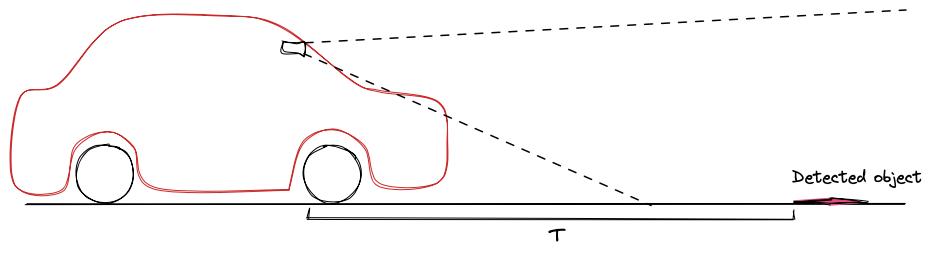
\includegraphics[width=0.95\textwidth]{images/1_introduction/setup-schema.png}
	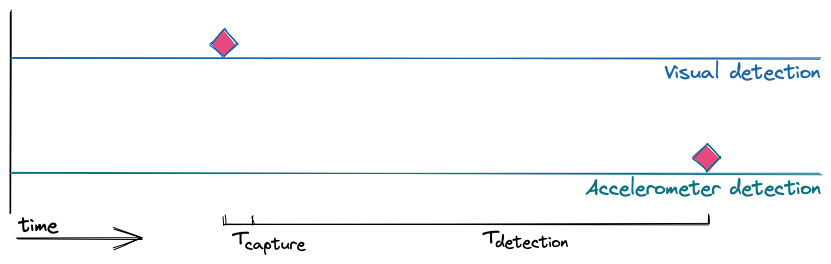
\includegraphics[width=0.95\textwidth,keepaspectratio]{images/2_literature/time-line-synchonization.png}
    \end{center}
    \captionsetup{width=.95\textwidth}
    \caption{Illustration of the setup of collecting data.}
    \label{fig:time-synchronization}
\end{figure}




\subsection{Research Questions}

During this research, data is continuously collected from driving on roads. In particular, it is collected by a smartphone with a customized app, which collects GPS, accelerometer, and video data that need to be combined. Visual data can only be recorded in decent conditions i.e., it depends on weather and lighting. Complementary, vibrations can always be measured regardless of external conditions. At the same time, interpreting vibration data is a more difficult task for humans. Combining both data sources helps to interpret the data. With these points in mind, this thesis aims to answer the following research question:

\begin{itemize}
\item \textbf{RQ: To what extent can visual object detection and accelerometer data be combined in a multimodal machine learning pipeline to correctly classify road surface anomalies?}
\end{itemize}

To answer this question, we divided the question into smaller parts. From quick literature survey, it is known that research exists on classifying road surface defects on single source of data. As the aim is to combine visual- and accelerometer data, it makes sense to first research what is known for each respective source in the field of road surface defect detection. Detecting defects using visual data is basically object detection: localization and classification of objects (i.e., damages) in an image. The first two sub research questions are:

\begin{itemize}
\item \textit{SQ1: What is the state of art in machine learning pipelines using object detection to classify road surface anomalies?}
\item \textit{SQ2: What is the state of art in machine learning pipelines using accelerometer data to classify road surface anomalies?}
\end{itemize}

Combining visual and accelerometer data only works when both sources are synchronized correctly. As previously mentioned, the problem is that the same event (i.e., defect) is registered with some delay $\tau$ between the data sourced, see figure \ref{fig:time-synchronization} above. In order to correctly combine these sources, we need to find a method to calculate this delay. Therefore the last sub research question is:

\begin{itemize}
\item \textit{SQ3: How can visual data and accelerometer data be synchronized?}
\end{itemize}

To answer this question, a novel method is designed to automatically calculate this delay. With the synchronized sources, we test the combined pipeline. The final answer to the RQ is evaluated based on the empirical results. When we observe that the classification accuracy of the pipeline with combined data is higher than that of either unimodal pipeline, we can conclude that combining the sources was successful. If the accuracy is lower, we need to dig into the data to understand how future research can address this problem.


\subsection{Contributions}

TODO

This thesis provides interesting contributions, both scientifically from the performed research, and business value from the developed application. First of all, this is the first research to combine both visual and accelerometer data to detect road surface anomalies. Especially interesting is the steps undertaken to synchronize both data sources. The effect of combining sources is rigorously evaluated by comparing the difference in accuracy between combined pipeline and of the respective unimodal pipelines. 

The application yields large business value for the company. 


\subsection{Remainder}

TODO

The remainder of this thesis is structured as follows:

\begin{enumerate}
\addtocounter{enumi}{1}
\item \textbf{Literature} presents the current literature known on the subject. It answers the theoretical research subquestions 1-3. 
\item \textbf{Methodology} explains the methodology that is used during this thesis.
\item \textbf{Data Processing} presents the various data engineering activities required to record and process the data in order to make predictions.
\item \textbf{Multimodal Fusion} deals with the performed experiments.
\item \textbf{Discussion} interprets the results.
\item \textbf{Conclusion} concludes the thesis, and provides some suggestions for future activities.

\end{enumerate}

